%\chapter{U--\protect\NoCaseChange{Mo} fuel: a brief introduction}
\chapter{Introduction}
Since the discovery of fission in 1938, the world has experienced the impact of nuclear power on modern society. The primary fuel for fission is $^{235}$U . Naturally occurring uranium consists of a combination of different isotopes; about 99.3\% $^{238}$U,  0.7\% $^{235}$U and trace amounts of $^{234}$U isotope. Uranium can be ``enriched'' in the $^{235}$U isotope by using various complicated processes that mainly uses the difference in masses and/or other physical properties. A typical power generating reactor requires less than 5\% enriched uranium. Research reactors needs a higher percentage of enriched uranium. The primary purpose of a research reactor is to produce neutron. The neutron produced by a research reactor are used for neuttron scattering, testing and analysis of materials, production of radioisotopes, and training.
 They are also referred as non-power reactors.

%Uranium that has a concentration of $^{235}$U from natural level to 20\% is called low enriched uranium (LEU). Typical power reactor fuel has $^{235}$U assays below 5\%.

After the Manhattan project, the highly enriched uranium ($>$ 90\% $^{235}$U) has been used peaceful in scientific research and radioisotope production. Nuclear fuels are characterized by a unique combination of physics, engineering, safety requirements, social and environmental factors, and international concerns. The purpose of nuclear safety is to prohibit the uncontrolled release of the radioactive isotopes to the environment and ensuring safe use of the fissile material. Highly enriched uranium (HEU) fuel is also a proliferation concern. All enrichments above 20\% $^{235}$U are considered HEU~\cite{international2005iaea}.

HEU can be used to make simple nuclear explosives, such as the one used in Hiroshima by the United States. That weapon code named ``little boy'', contained about 50 kilograms of $^{235}$U with an average enrichment of about 80\%~\cite{serber1992alamos}. The neutron production in 60 kg of metallic enriched uranium (from both fission and (\textalpha, n) reactions on oxygen) is about 100 per second. This low rate and combined with a neutron reflector can be made into simple highly-enriched uranium weapon. Although there are counter arguments about the likelihood of acquiring necessary technical capabilities to make an implosion design, there is little argument that it is much easier to design a so called gun-type weapon that could in theory work without testing. Stocks of HEU fuel at research reactors and in their nuclear fuel cycles are particularly vulnerable to theft.

%\section{Introduction}\label{sec_ch1_intro}
Proliferation concerns about HEU resulted in a global effort, led by the USA, to eliminate the civil uses of HEU in research and test reactors. One of the important HEU reduction programmes is known as the Reduced Enrichment for Research and Test Reactors (RERTR). The RERTR program was initiated in the USA in the late 1970s to develop new nuclear fission fuels to replace high-enriched uranium (HEU)~\cite{travelli1980current,snelgrove1997development}\@.  The RERTR program is now managed by the U. S. National Nuclear Security Administration's (NNSA) Office of Material Management and Minimization~\cite{burkes2021thermal}. The development of low-enrichment uranium (LEU) fuels for high-performance reactors is an important nonproliferation initiative.

This initiative has completed a total of 69 reactor conversions to use LEU fuel, and 26 HEU-based reactor facilities have been verified to have been shut down~\cite{wilson2017us}. The conversion of six domestic high performance research reactors\footnote{Advance Test Reactor (ATR) at INL, Idaho; Advanced Test Reactor Critical (ATRC) Assembly at INL, Idaho; High Flux Isotope Reactor (HFIR) at ORNL, Tennessee; Massachusetts Institute of Technology Reactor (MITR), Massachusetts; National Bureau of Standards Reactor in Gaithersburg, Maryland; University of Missouri Research Reactor (MURR) in Columbia, Missouri.} that still use highly enriched uranium fuel is yet to be achieved. Due to their unique operating conditions, converting these six reactors will not be easy and a plethora of nuclear engineering challenges are associated with their conversion. These conversion process may take longer time periods, but developing a new LEU fuel is essential to ensure better performance and limiting nuclear proliferation. The timeline for the conversion is currently estimated to be 10--16 years~\cite{national2016reducing, national2012progress, kaufmann1962nuclear}. 


Research reactors operate at relatively low peak fuel temperatures, but are required to meet fuel performance requirements at high burnup. A typical peak fuel centerline temperature in a research reactor is around 250\textdegree C~\cite{meyer2014irradiation}. For a research reactor, fission densities are usually in the range of $3\times10^{21}$ to $6\times10^{21}$ fissions/cm$^3$. In some cases, peak fuel fission density exceeds $7\times10^{21}$ fissions/cm$^3$, requiring a higher density of $^{235}$U atoms. Consequently, one of the main requirements of LEU fuels is increased uranium density, such as that found in metallic uranium, to offset the decrease in \textsuperscript{235}U enrichment. 

\section{Metallic Uranium and Alloys}
Uranium has three allotropic forms: orthorhombic (\textalpha-phase), stable from below room temperature to 662\textdegree C; tetragonal (\textbeta-phase), stable from 662 to 774\textdegree C; and body-centered cubic (\textgamma-phase), stable from 772\textdegree C to the melting point, 1132\textdegree C~\cite{kaufmann1962nuclear}. Metallic uranium at standard temperature is thought to have sufficient density ($19.05\pm0.02$ g/cm$^3$). \textalpha-U belongs to the orthorhombic system, in which the three axes are mutually perpendicular($a\perp b\perp c$) but are unequal length ($a\ne b\ne c$). This orientation of crystal is considered \textit{anisotropic}. As a result, a great deal of work has gone into studying the textures of alpha uranium. Different heat treatment, corrosion studies, grain size analysis, mechanical and elastic property studies and post irradiation analysis indicate that \textalpha-uranium has poor properties to be considered as nuclear fuel~\cite{pugh1961swelling, loomis1962swelling, chiswik1958osti}.

Alloying uranium to obtain certain properties was extensively studied in the early stages of nuclear fuel development. Some of the reasons being 1) to achieve a finer grain size, 2) to improve mechanical properties, 3) to improve corrosion resistance, 4) to increase irradiation performance etc. Aluminum is the material for choice for many components of low-temperature research reactors. The irradiation behavior of Al at low temperature ($<$100\textdegree C) shows favorable behavior, which retains significant ductility and metallic property~\cite{farrell2012}. The uranium-aluminum system has three compounds (Fig.~\ref{fig:ualphase}) -- UAl$_2$, UAl$_3$ and UAl$_4$. UAl$_2$ solidifies at temperature of 1615\textdegree C; UAl$_3$ forms at 1355\textdegree C by a peritectic reaction between the solid phase of UAl$_2$ and liquid phase of Al--60wt\%U. UAl$_4$ forms at 740\textdegree C by a peritectic reaction between the solid phase UAl$_3$ and the liquid phase of Al--18wt\%U. Uranium--aluminum alloys in which the matrix is either primary aluminum or Al+UAl$_4$ eutectic are widely being as research reactor fuel. This type of fuel is called \textit{dispersion}\footnotemark\@ fuel.

\footnotetext{A dispersion type fuel is one in which the fissile material is contained as a compound dispersed in a nonfissile matrix~\cite{white1957}}

Uranium-aluminum alloys can have density as high as 4.522 gU/cm$^3$~\cite{saller1956study}, for LEU the required density exceeds 8.5 gU/cm$^3$~\cite{sannen2014}. There are only a few fuel phases with both a high uranium density and stable irradiation properties. The two types of fuels that meet the density requirements are \textgamma-stable uranium and U$_6$Me (Me=transition metal) type compounds. The U$_6$Me type fuels showed very poor irradiation performance at low fission density (\num{3e21}fissions/cm$^3$)~\cite{meyer2000irradiation, hofman1987irradiation, vandenberghe2010}. The \textgamma-phase of uranium can be stabilized by alloying it with suitable elements. Several transition metals stabilizes \textgamma-U. Elements such as molybdenum (Mo), niobium (Nb), titanium (Ti), and zirconium (Zr) have been tried as alloying elements because of their solubility in \textgamma-uranium~\cite{donze1959stabilisation,giraud1973formation,lopes2013mechanical}. The U--Mo phase (Fig.~\ref{fig:umophase}) has a eutectoid decomposition of \textgamma-phase at 11.1 wt\% Mo and 555 \textdegree C. If the U--Mo \textgamma-phase contains more than 5--7 wt\% Mo, the \textgamma-phase is retained at room temperature by rapid cooling~\cite{saller1954transformation, bostrom1957}.
 To take advantage of this, uranium alloyed with 10 wt$\%$ molybdenum (U-10Mo) is currently being developed as a potential high-density LEU fuel for high-performance research reactors~\cite{prabhakaran2017u, meyer2014irradiation, williams2017post}. 
%Uranium alloys that retain the high-temperature \textgamma-phase, which is body-centered cubic, are more suitable for reactor fuel due to their more isotropic radiation-induced swelling behavior compared with  \textalpha-uranium~\cite{kittel1993history}.

\begin{figure}
\centering
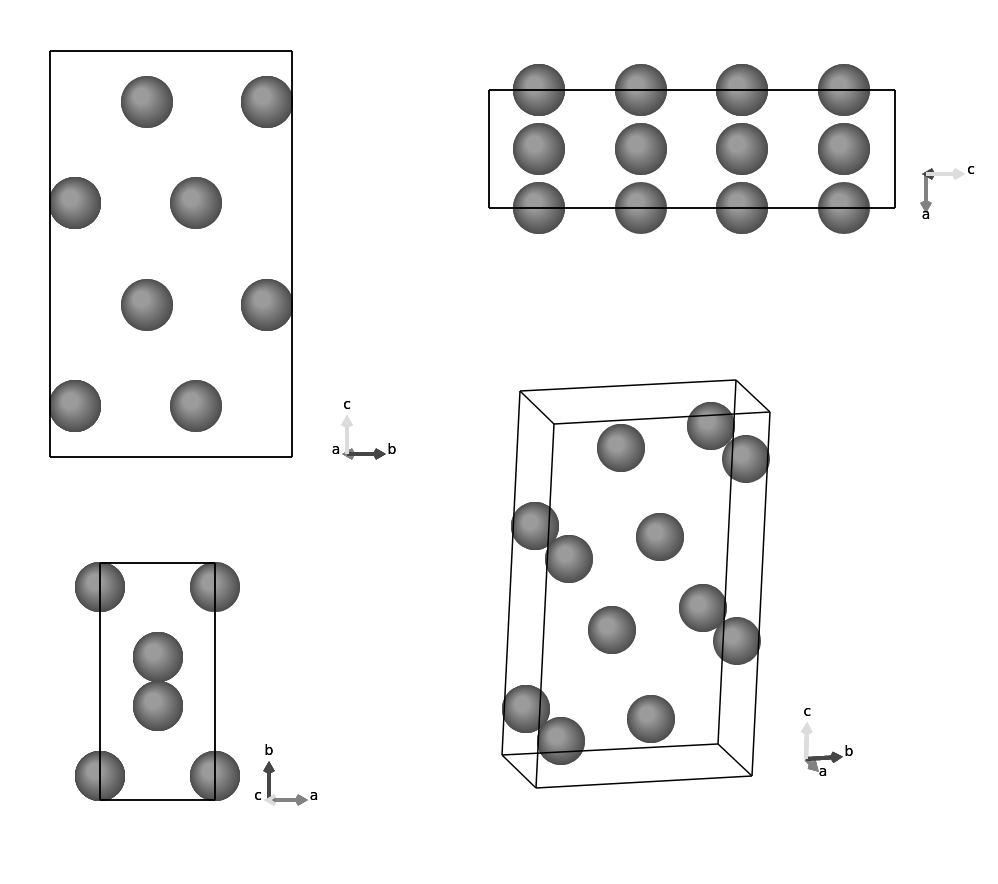
\includegraphics[scale=1.2]{4_image_alphs_greyscale}
\caption{Orthorhombic crystal structure of \textalpha-uranium}
\end{figure}

%The U-Mo alloy has been identified as a high-performance fuel due to its high uranium density and low neutron capture cross-section~\cite{ewh2010microstructural,smirnova2013ternary,rest2009analysis,landa2013density}.


\begin{figure}
\centering

\includegraphics[width=4.5 in]{u-mo-phase-diagram}
\caption[U--Mo phase diagram]{Uranium--Molybdnum phase diagram. Image reprinted with permision from Okamoto~\cite{okamoto2012mo}}
\label{fig:umophase}
\end{figure}

\begin{figure}
\centering
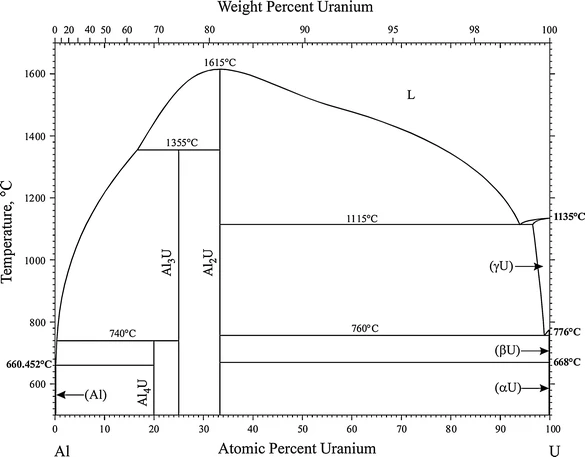
\includegraphics[width=4.25 in]{images/u-al-phase-d.png}
\caption[U--Al phase diagram]{Uranium--Aluminum phase diagram. Image reprinted with permission from Okamoto~\cite{okamoto2012mo}}
\label{fig:ualphase}
\end{figure}



Before the current interest in U--Mo metallic fuel, some of the early nuclear reactors used metallic fuel because of the combination of high uranium density and metallic properties. The Godiva IV pulsed reactors at Los Alamos (initially known as \textit{Lady Godiva}) used U--Mo alloys, which date back to 1960. The Fast Burst Reactor (FBR) at White Sands, the Army Pulsed Radiation Facility (Aberdeen, MD), and the Sandia Pulsed Reactor II also used U--Mo alloys. All of these reactors utilized the \textgamma~phase of uranium, but because of the short irradiation time, the impacts of fuel burnup were minimal~\cite{horak1973operating}. The Dounreay Fast Reactor used a number of metal-fuel-based designs, which inclueds U--9.1Mo (9.1 wt\% Mo) and U--7Mo clad in niobium. The highly alloyed fuel cracked more, even though the U--9.1Mo fuel swelled slightly less than U--7Mo alloy~\cite{cottrell1964development}. In U.S. the Enrico Fermi Fast Breeder Reactor (EFFBR) was the first commercial fast reactor that used U--10Mo fuel. 

The primary concern was to ensure that the fuel would remain in the \textgamma-phase during the operating condition. A series of experiments have been performed to map the fission rate and temperature dependence of the \textgamma-phase's stability~\cite{no20031374}. Two types of U--Mo alloy fuel have been designed and tested. One is monolithic fuel, in which a thin layer of U--Mo foil is bonded to aluminum cladding. The other is a dispersion fuel in which of U--Mo fuel particles are dispersed in an Al matrix.



For five decades, dispersion fuels have powered many test and research reactors worldwide. The manufacturing process and operating conditions are well established for these types of fuels. High-burnup testing of dispersion fuels showed a pattern of \mbox{breakaway} swelling\footnotemark\@ behavior at intermediate burnup. The post-irradiation examination of the U--Mo dispersion fuel revealed that this phenomenon is related to the formation of ternary aluminide phase. Reaction between the U--Mo fuel kernels and aluminum cladding occurs during irradiation and forms a ternary [(U--Mo)Al$_x$] phase which releases the fission gas at the boundary between the interaction phase and the aluminum matrix~\cite{leenaers2004post,jue2014microstructural,van2008transmission, olander2009growth}. These gas bubbles have a tendency to aggregate into the gas pockets, which weakens the fuel meat by exerting internal pressure. The result is mechanical failure and increase in fuel volume. To eliminate the fuel--matrix interaction, a `monolithic' U--Mo fuel was suggested. In monolithic fuels, a zirconium foil is used as a diffusion barrier between the fuel and the cladding (aluminum) to prevent diffusion of molybdenum into the cladding~\cite{jue2014microstructural}.

\footnotetext{\textit{Breakaway} is defined as ``the limiting exposure, beyond which there will be a marked increase in the rate of swelling as a function of burnup~\cite{osti_10163384}"}.



\section{Fission Gas}
The behavior of fission products xenon and krypton has perplexed and fascinated both the experimentalists and theorists more than many processes simultaneously occur in a nuclear fuel element during irradiation. These inert gases are insoluble in fuel matrix, causing them to form small gas bubbles. If the gas is released from the fuel, the pressure within the fuel pin rises and that ultimately results in failure. If the fission gases are retained in the fuel, however, they almost always precipitates as bubbles and causes swelling in the fuel matrix. Swelling adversely impact the fuel efficiency. It impacts the thermal conductivity of the fuel thereby disrupts the efficient heat extraction from the fuel. One particular xenon isotope, $^{135}$Xe has a large neutron absorption cross section which can lead a reactor poisoning. As a result the basic aspects of inert gas behavior were studied for fuel such as UO$_2$.

Xenon is produced directly from fission. 0.3\% of the fission products are $^{135}$Xe. It is also produced by the decay of $^{135}$I via the following scheme:

\begin{equation*}
\ce{^{135}Te ->[$19 \text{s}$] ^{135}I ->[6.7h] ^{135}Xe}
\end{equation*}

$^{135}$I constitutes almost 6.1\% of fission products. Thus, 95\% of the total xenon production is due to the decay of iodine. Xenon is removed from the reactor by a beta decay or by neutron absorption:
\begin{equation*}
\ce{^{135}Xe ->[9.1 $\text{hr}$] ^{135}Cs + $\beta$}
\end{equation*}

In U--Mo fuel fission gas forms bubbles  both inside the grain and in to the grain boundary. In side the grains fission gas forms superlattices~\cite{miller2012advantages, gan2010transmission}. 

This dissertation investigates how fission gas (xenon and krypton) impacts the transport properties of U--Mo fuel. Chapter~2 summarizes theoretical methods used in this work. In Chapter~3, We discuss the reduction of thermal conductivity due to the presence of fission gas. We have used finte element method to approximate the overall thermal conductivity. In Chapter~4, we introduce a new pseudopotential for metallic uranium to study the properties using density functional theory (DFT). In Chapter~5 we look into the diffusion mechanism of xenon in \textgamma-uranium and U--Mo alloy. In Chapter~6, we discuss the conclusions and potential future work.


%In the current work we have investigated how fission gas (xenon and krypton) impacts the U--Mo fuel. In the second chapter we have studied the reduction of thermal conductivity due to the presence of xenon gas. We have implemented finite element method to study the different microstructural configuration of fission gas in U--Mo fuel. In the third chapter we have introduced a new \textit{pseudopotential} for metallic uranium to study the properties using first-principles (Density Functional Theory (DFT)) method. In the fourth chapter we will discuss about the atomistic diffusion mechanism of xenon in U--Mo fuel, which includes the study of xenon gas in the U--Mo fuel using DFT methods. 
















\bibliographystyle{apsrev4-1}
\bibliography{abbreviated,comp}
